\chapter{Background}

In this chapter, concepts and terminology relevant to the thesis is explained, mainly, technological foundations such as \acrfull{ais}, conceptual foundations such as \acrshort{ais}-based trajectories and trajectory similarity measurements, and techniques applied to predicting future destination ports of traveling vessels, namely, \acrfull{ml}.

\section{Concepts}

This section describes the broader concepts that are important to the thesis's solution and later discussions,

\subsection{Vessel voyage definition}

In order to effectively predict a vessel's future destination, or analyze voyage patterns in general, a vessel voyage must first be defined. This is a crucial concept to define as it would change the outcome of any prediction method that considers historical voyages. The main factor to decide on is when does a vessel arrive at a port, or what conditions must be true for a vessel to have arrived at a port.

There might be several different reasons for a vessel to visit a port, not all of which means that the port was the vessels final stop in a voyage. For instance, larger vessels traveling long distances, often have to bunker (refuel) at bunker ports between the port they loaded and the port they will unload at. In some cases, vessels anchor outside of such bunker ports awaiting to be refueled by bunker vessels, while in other cases they can reduce their speed and be refueled without ever stopping completely. Another common reason for vessels to physically stop moving is congestion in ports. Very often vessels of any size have to wait their turn before loading or unloading at busy ports. In these cases they might anchor closer to a different port while they wait for access, however, it is likely that they do not consider themselves arrived in these scenarios. In either case, whether vessels refueling at bunker ports, or stopping for other reasons, should be considered arrivals or not ultimately depends on the desired outcome of future predictions and context.

For the purpose of this thesis, a voyage is defined only when the vessel herself claims to be moored by reflecting this as a navigational status in the \acrfull{ais} data. As vessels usually do not use the moored signal when bunkering, or for short stops along a voyage, this entails that the proposed solution will be more prone to predicting the final destination of a vessel even though it might stop for other reasons along the voyage. This voyage is beneficial for actors in the industry who are interested in knowing what vessels are available in different regions for chartering, however, a disadvantage is that fewer voyages can be constructed from the available data as longer voyages could have been divided into multiple smaller voyages if considering, for instance, bunkering as port arrivals.


\subsection{Trajectory similarity}

As will be further elaborated on in \cref{chap:related_work}, the current literature related to vessel destination predictions almost exclusively rely on some form of trajectory similarity. Therefore, trajectory similarity is also included in this thesis' proposed approach to vessel destination prediction. There are three main categories of trajectory similarity measurements: spatial, temporal, and tempo-spatial. Regarding vessel trajectories derived from \acrshort{ais}, they are not likely to share similar time intervals values as vessels travel at different speeds and at different times, therefore, for the purpose of this thesis, only spatial trajectory similarity measures are considered. This assumption is further corroborated by \cite{Zhang2020AISApproach} that arrived at a similar conclusion in their work developing a \acrfull{ml} -based approach to trajectory similarity measurements.

There are a number of spatial trajectory comparison methods that have been widely used for different purposes. The most relevant are the Hausdorff distance \parencite{magdy2015}, Fréchet distance \parencite{magdy2015}, and \acrfull{sspd} \parencite{besse2015review}. Out of these, the \acrshort{sspd} method is the most appropriate as it handles trajectories of different shapes and lengths well which is beneficial when comparing a trajectory from an ongoing vessel voyage to a set of complete historical ones. \cref{fig:sspd} shows an example from \cite{besse2015review} where two trajectories are compared and their symmetric distances are calculated.

\begin{figure}[htbp]  % order of priority: h here, t top, b bottom, p page
    \centering
    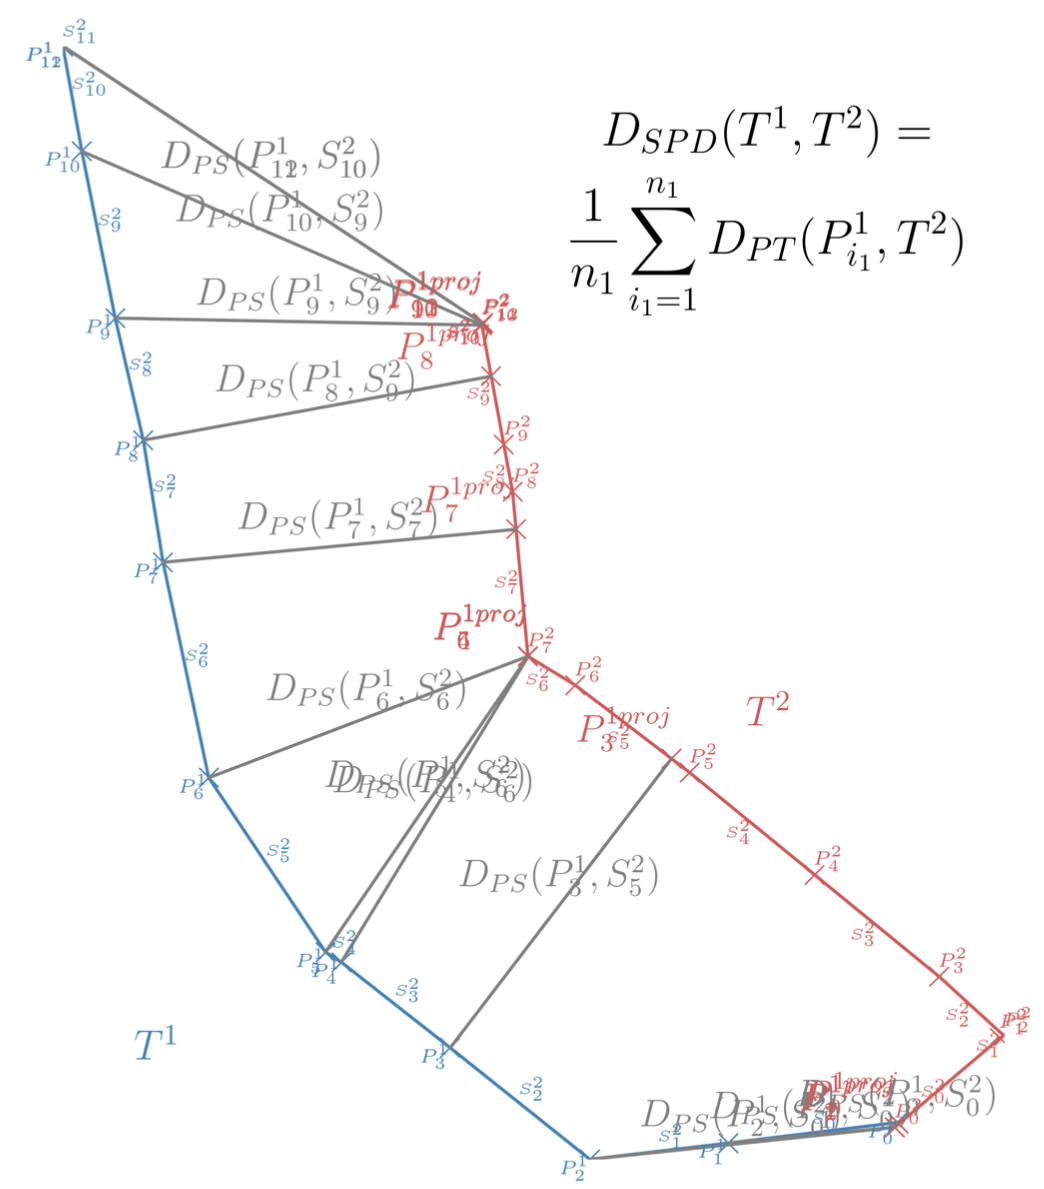
\includegraphics[width=0.5\textwidth]{figures/sspd}
    \caption{Segment Path Distance (SPD) in the SSPD process of comparing two different trajectories \parencite{besse2015review}}
    \label{fig:sspd}
\end{figure}

The methods mentioned thus far are all algorithmic approaches to measuring similarities between trajectories, however, there are also \acrshort{ml}-based methods as well such as the approach proposed in \cite{Zhang2020AISApproach} that also compares their results to the aforementioned methods. They used a \acrfull{rf} to measure similarities between a traveling trajectory and every historical trajectory traveling from the same departure port in order to predict the next destination port for a vessel. They achieved a higher general accuracy when compared to algorithmic methods such as \acrshort{sspd}. Moreover, for similar purposes, some unsupervised clustering methods have also been applied to similar problems such as the \acrfull{dbscan} which is capable of sequentially finding patterns in points and trajectories. This approach is more frequently used in trajectory predictions on a small geographical extent such as for collision detection and anomaly detection.

\subsection{Machine learning (ML)}

\acrfull{ml} is an umbrella term describing computer algorithms that automatically adapt and improve based on experience. There is a vast number of different \acrshort{ml} algorithms applied to different problem areas. \acrshort{ml} is mainly divided into three broad categories: supervised learning, unsupervised learning, and reinforcement learning. In supervised learning, in the training process, both input and the desired output are provided to the model. The model finds patterns and correlations between input and output data during the training process, and when the model is trained or fitted, it is capable of guessing output given only input. In unsupervised learning, no output labels are provided to the model leaving the model to find patterns in the input set on its own. Clustering is an example of unsupervised learning as the model finds and labels patterns in input data without any external guidance. Reinforcement learning is a dynamic approach to \acrshort{ml} where the model continuously learns while trying to achieve a goal. In this method, the model navigates a problem space, and the program rewards or punishes the model that tries to optimize for rewards. In regards to topics covered by this thesis, \acrshort{ml}-based trajectory comparisons involve unsupervised learning, while predicting destination ports is supervised as the historical destinations are known.

\begin{figure}[htbp]  % order of priority: h here, t top, b bottom, p page
    \centering
    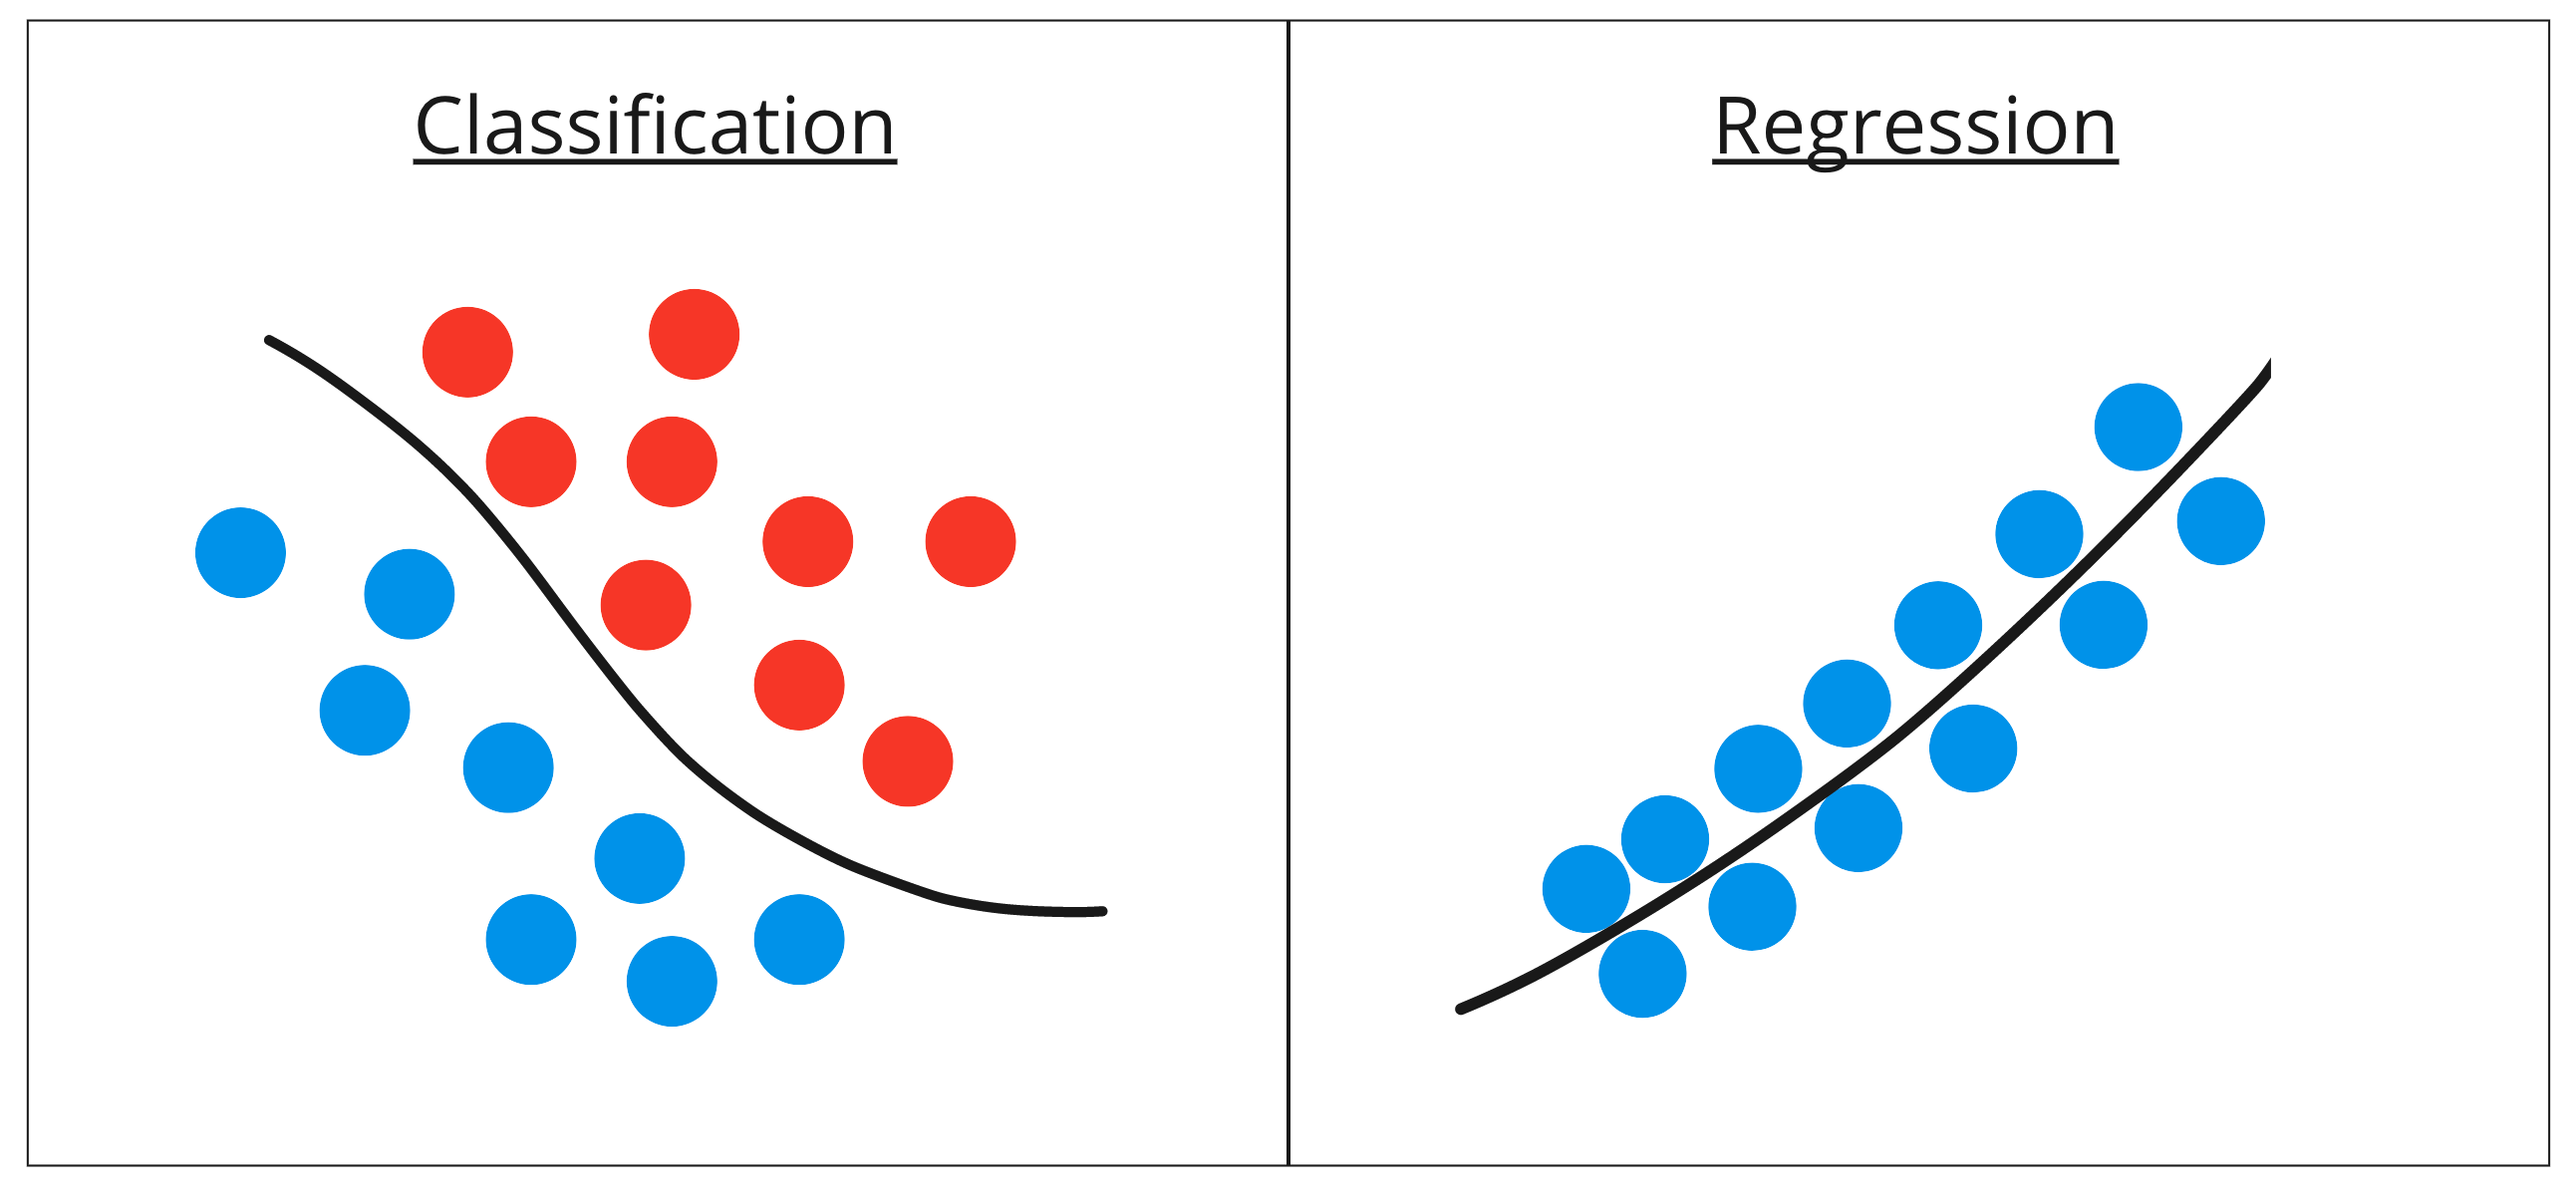
\includegraphics[width=0.75\textwidth]{figures/class_regg}
    \caption{Example showing the difference between classification and regression tasks}
    \label{fig:classification_regression}
\end{figure}

Moreover, supervised learning can further be divided into regression and classification problems. The main difference between the two is that classification aims at predicting a label, or a class, while regression predicts a quantity that is not necessarily present in the training data. For instance, a regression model can be used to predict the price of an item for sale, while classification can be used to label emails as "spam" or "not spam". \cref{fig:classification_regression} shows the difference between classification and regression. The example of classifying emails as ``spam'' or ``not spam'' would be considered a binary classification problem as there are only two possible labels, however, classification can also involve predicting more than two outcomes which is commonly referred to as multi-class classification. In the context of this thesis, predicting a vessel's destination port can be formulated as a multi-class classification problem as every possible destination port are different possible labels for a given voyage in progress. \cref{fig:ml_terms} shows the how \acrshort{ml} is hierarchically divided into more specific terms relevant for the scope of this thesis.

\begin{figure}[htbp]  % order of priority: h here, t top, b bottom, p page
    \centering
    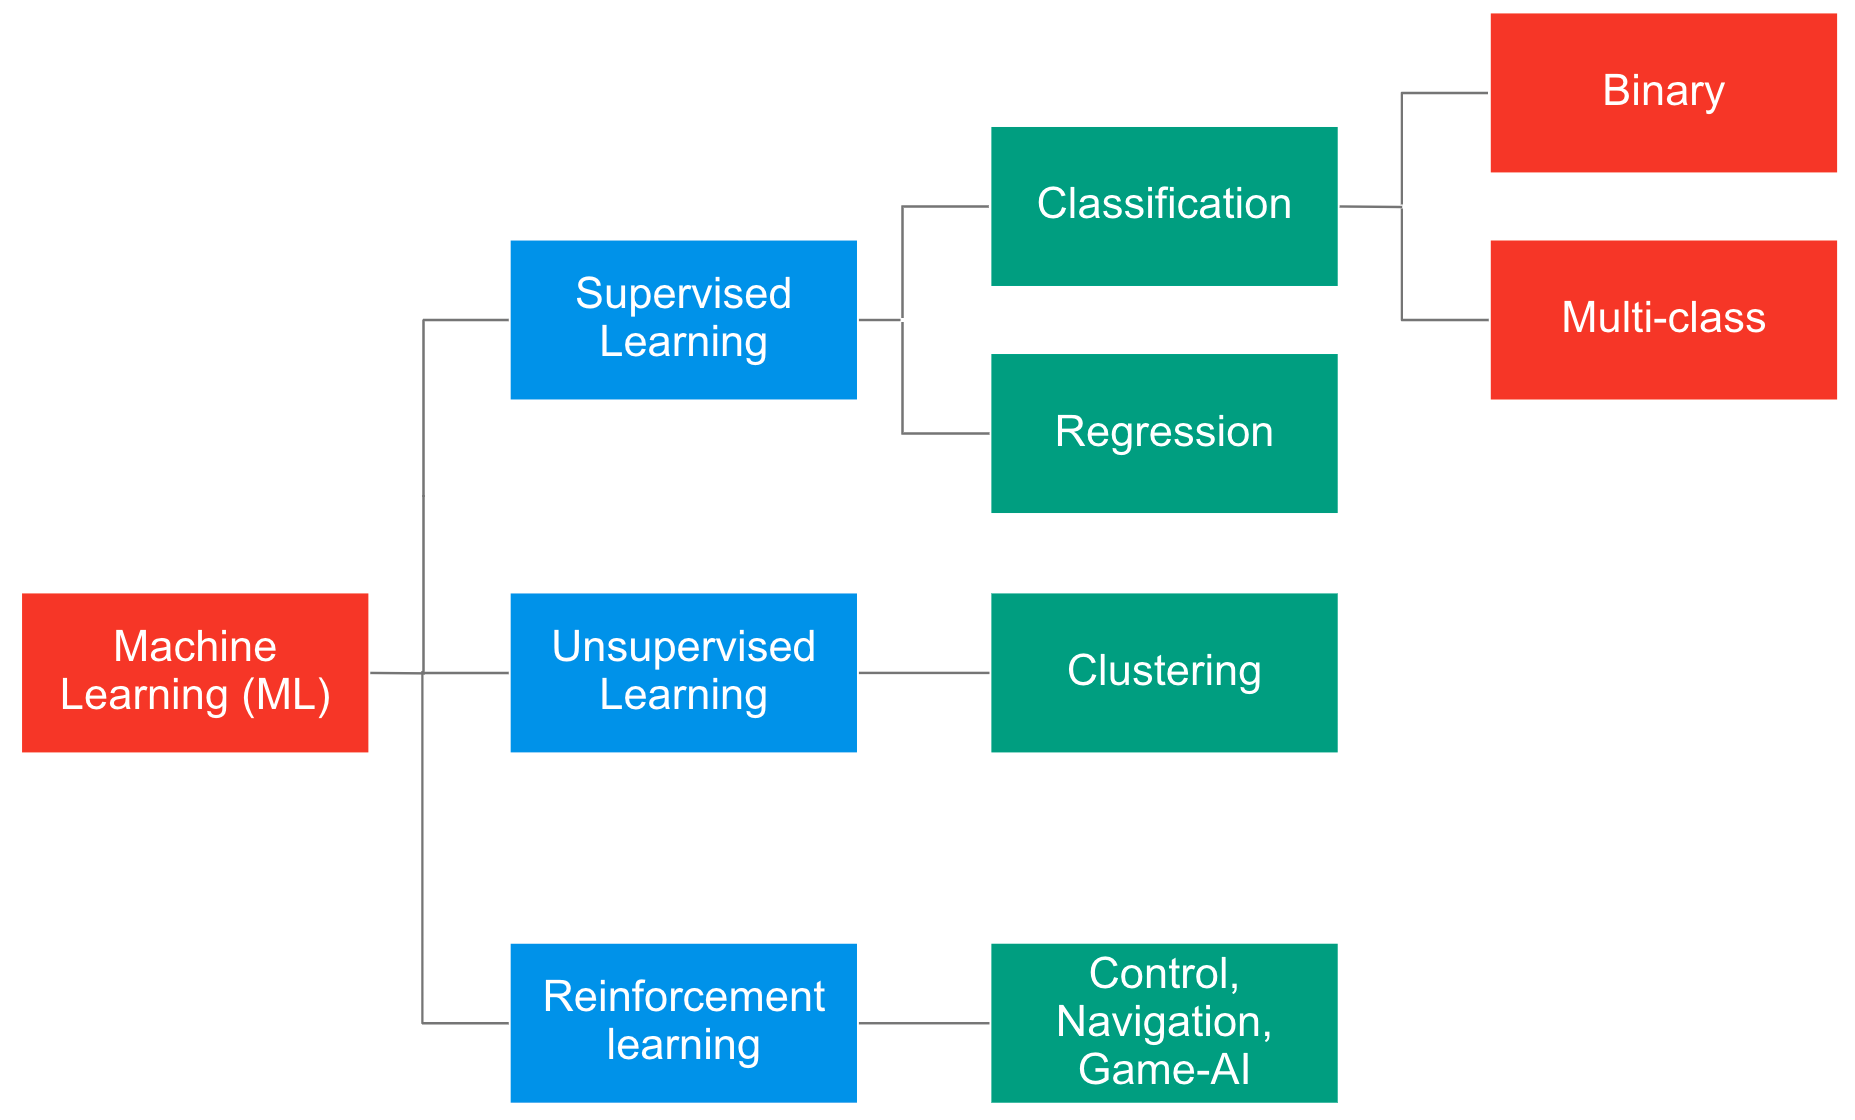
\includegraphics[width=0.75\textwidth]{figures/ml-terms}
    \caption{Machine Learning (ML) hierarchical terminology}
    \label{fig:ml_terms}
\end{figure}

\begin{itemize}
    \item Cross-validation
    \item Hyperparameter optimization
\end{itemize}

\section{Technologies and protocols}

\subsection{Database system}

All the data that is used throughout this thesis for analysis is collected and stored in a \textit{PostGreSQL} database. \textit{PostGreSQL}, or \textit{Postgres}, is an open-source object-relational database management system that supports the extended subset of SQL standards. One major advantage of using \textit{Postgres} is the support for plugins such as \textit{PostGIS} that provides tools for dealing with \acrshort{gis} and geometric data. In this thesis, \textit{PostGIS} is frequently used to store and process geographical trajectory data for vessel voyages. Throughout this thesis, when referring to the proposed methodology and results, terms such as database, table, row, and column refers to the \textit{PostGreSQL} database used and its tables with rows, and columns.

\subsection{Automatic Identification Systems (AIS) data}
\label{sec:ais_data}

\begin{figure}[htbp]  % order of priority: h here, t top, b bottom, p page
    \centering
    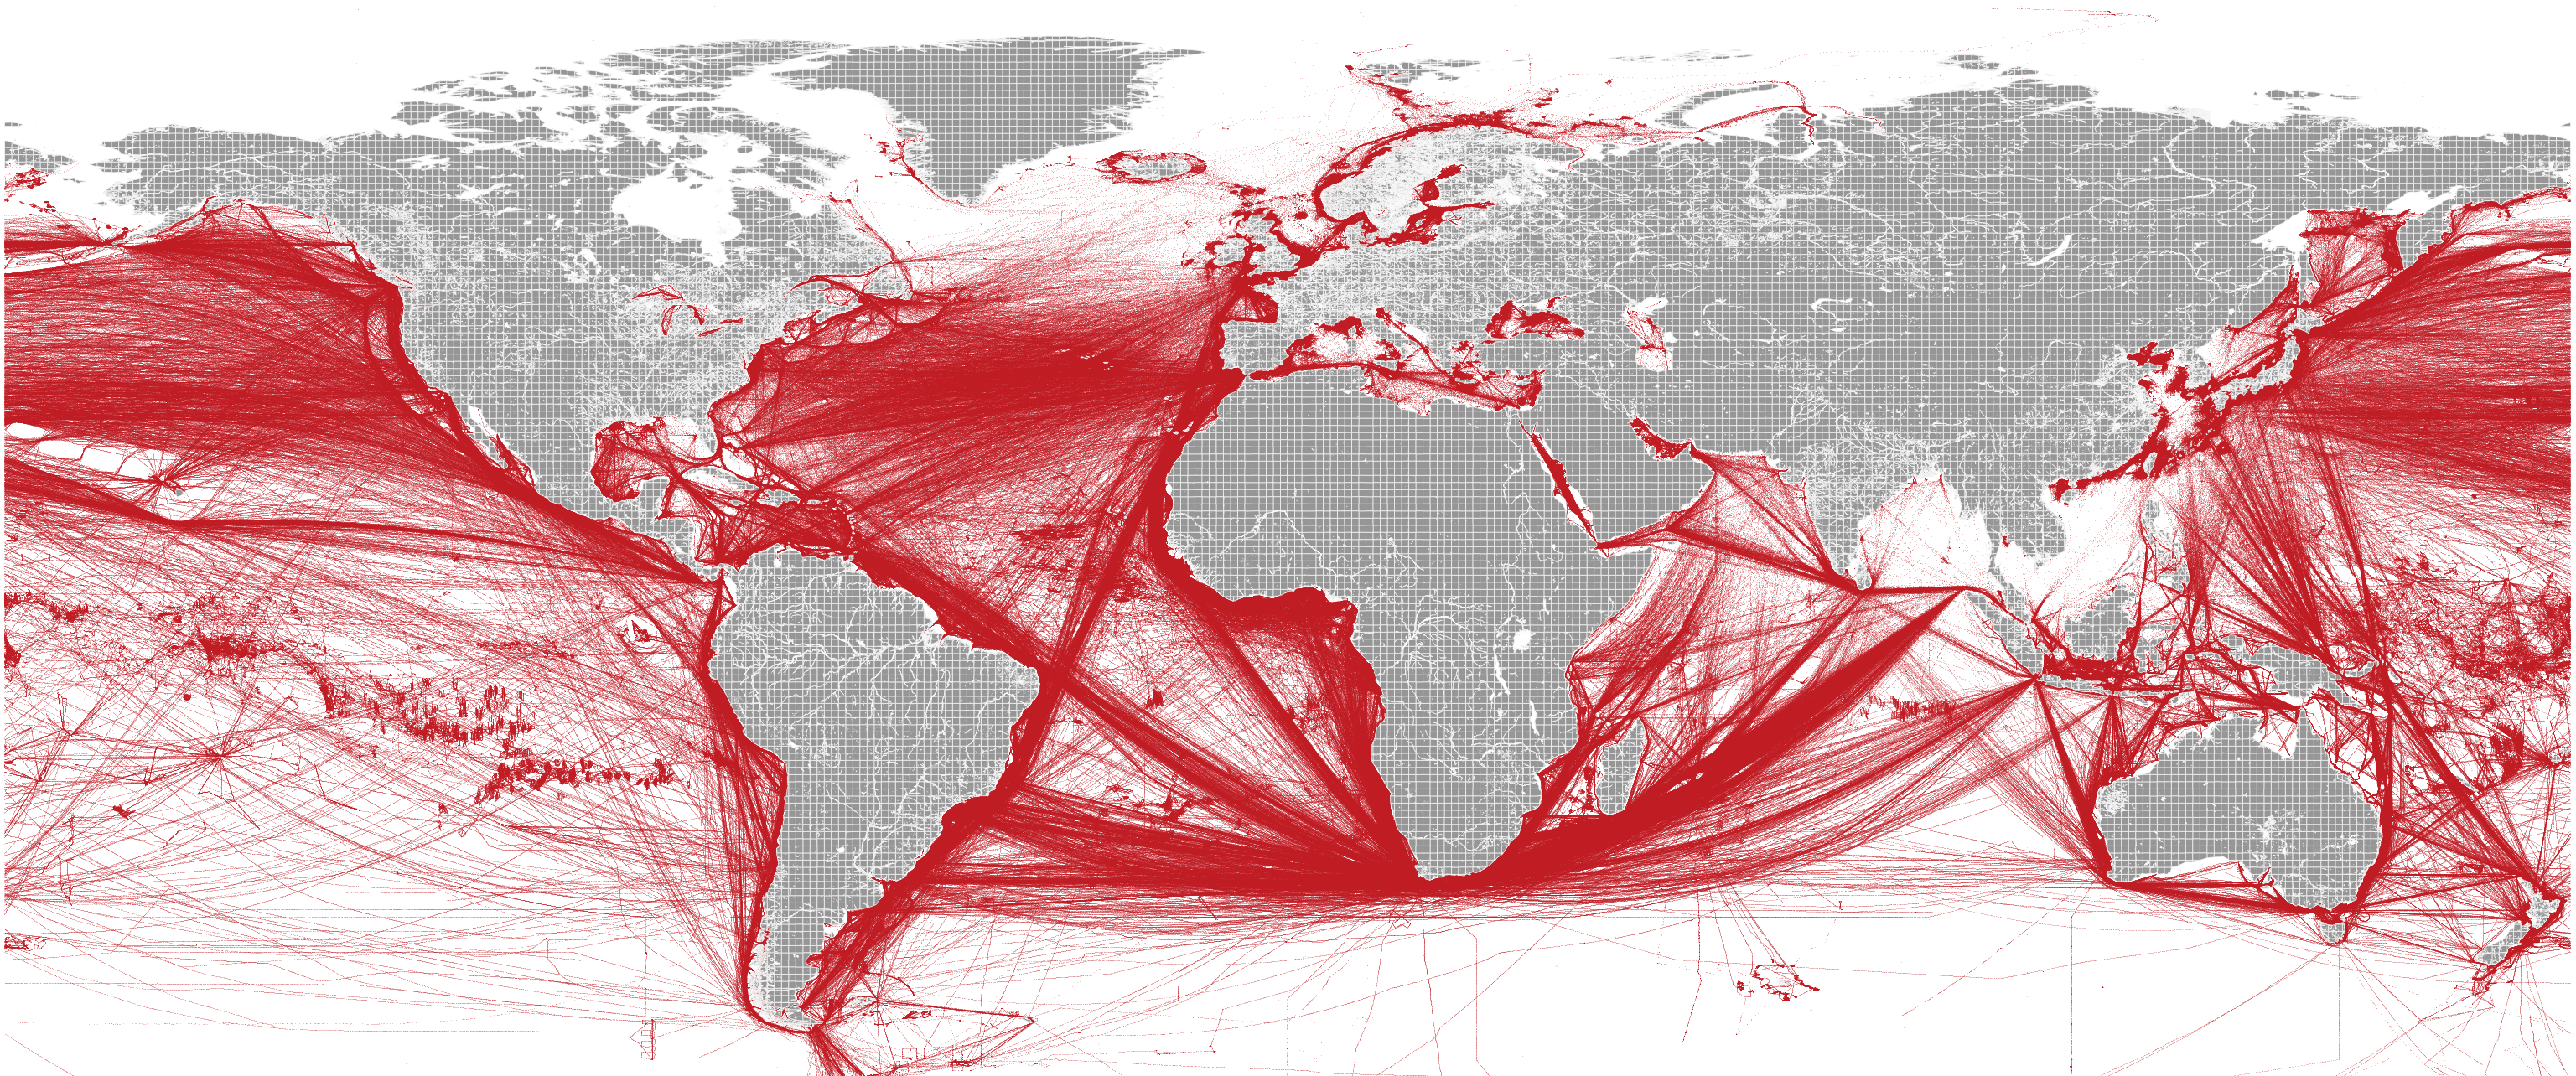
\includegraphics[width=1.0\textwidth]{figures/ais_history}
    \caption{Vessel positions derived from 100 million AIS positional reports}
    \label{fig:ais_positions}
\end{figure}

As already mentioned in \cref{sec:topics_covered}, \acrfull{ais} was initiated by \acrfull{imo} and since 2004 every commercial and passenger vessel exceeding 299 \acrfull{gt} is required to carry an \acrshort{ais} transmitter. These transmitters broadcasts \acrshort{ais} messages following the \gls{aivdm} protocol. The \gls{aivdm} protocol contains two main types of reports: positional and static. The positional reports contains automatically collected information such as the transmitting vessel's \acrfull{mmsi} number, the current timestamp, and the vessel's current navigational data including the current geographical coordinates, \acrfull{sog}, \acrfull{cog}, true heading, \acrfull{rot}, and more. The static reports contain additional information about the vessel and its current voyage, some of which are manually inputted, such as the vessel's \acrshort{imo} number, name, dimensions, draft, intended destination and \acrfull{eta}. As an example, \cref{fig:ais_positions} shows a visualization of 100 million \acrshort{ais} randomly chosen positional reports from a collection of historical \acrshort{ais} positions for global collection of shipping vessels. In relation, the historical \acrshort{ais} dataset used in this thesis consists of more than one billion records ranging from December 2019 to February 2021.

Regarding vessel identification in the \gls{aivdm} protocol, there are mainly two values that are unique to a given vessel: the \acrshort{mmsi} and \acrshort{imo} numbers. Either of these should be unique on their own for a given vessel, however, \acrshort{mmsi} numbers can be recycled under certain conditions such as when a vessel is put out of commission while the \acrshort{imo} number is specific to a vessel's hull. Therefore, \acrshort{imo} is the preferred identifier, however, since the \gls{aivdm} protocol divides these identifiers into positional and static reports, both need to be considered in order to use both static and positional \acrshort{ais} information.

\section{Initial data foundation}

This section describes the form and meaning of the data that forms the foundation of the thesis' proposed solution. The data is provided by the collaborative company \acrfull{mo} to the author.

\subsection{Vessel departure and arrival detection}
\label{sec:vessel_transitions}

\acrshort{mo} collects live \acrshort{ais} messages provided by a few sources, and in addition, they keep track of their navigational statuses as they are transmitted in the \gls{aivdm} protocol. These status attributes describe the current navigational state of the vessel for purposes of planning and security. Implicitly, these messages can indicate that a vessel has arrived or departed from a given port which can be used to detect voyages. When a vessel has concluded her journey and arrives at a port, the navigational status is changed to \textit{"MOORED"}, and when departing a port, the status is changed to \textit{"UNDERWAY USING ENGINE"} or \textit{"UNDERWAY SAILING"}. There are also other navigational statuses that could be relevant for voyage information such as \textit{"AT ANCHOR"} which could indicate that a vessel is bunkering (refueling) or is waiting for access to a berth that is congested. Currently, transitions from a status that indicates that a vessel is moving to the status \textit{"MOORED"}, and from \textit{"MOORED"} to moving are collected and labeled as arrivals and departures from or to the closest port within a given radius. This has proven to be a good method of identifying voyages and voyage trajectories between two ports as positions transmitted between a departure and arrival can be collected into a voyage trajectory that can be compared to other trajectories for analytical purposes. Throughout this thesis, this concept is referred to as vessel transitions.

\subsection{Additional vessel information and segmentation}
\label{sec:vessel_info_segments}

\acrshort{mo} has implemented a system for categorizing vessels into different segments, subsegments, and further variations. These segmentations are based on various factors such as the dimensional data provided by \acrshort{ais} messages as well as details provided by external vessel information sources and even user and manual input. The most important factors are the vessel type from the \gls{aivdm} protocol and the carry range, measured in \acrshort{dwt}, of the vessels which indicates how much cargo it can carry. This segmentation of vessels is highly relevant to voyage patterns as vessels of different types and sizes travel to different ports and countries for different shipping companies. This is further shown in \cref{fig:segment_map} which shows, from an image of \acrshort{mo}'s web platform, how different subsegments of the dry bulk cargo segment travels in different areas of the world. Since this categorization provides valuable insights into voyage patterns, vessel segmentation values are included in this thesis' proposed approach to vessel destination prediction.

\begin{figure}[htbp]  % order of priority: h here, t top, b bottom, p page
    \centering
    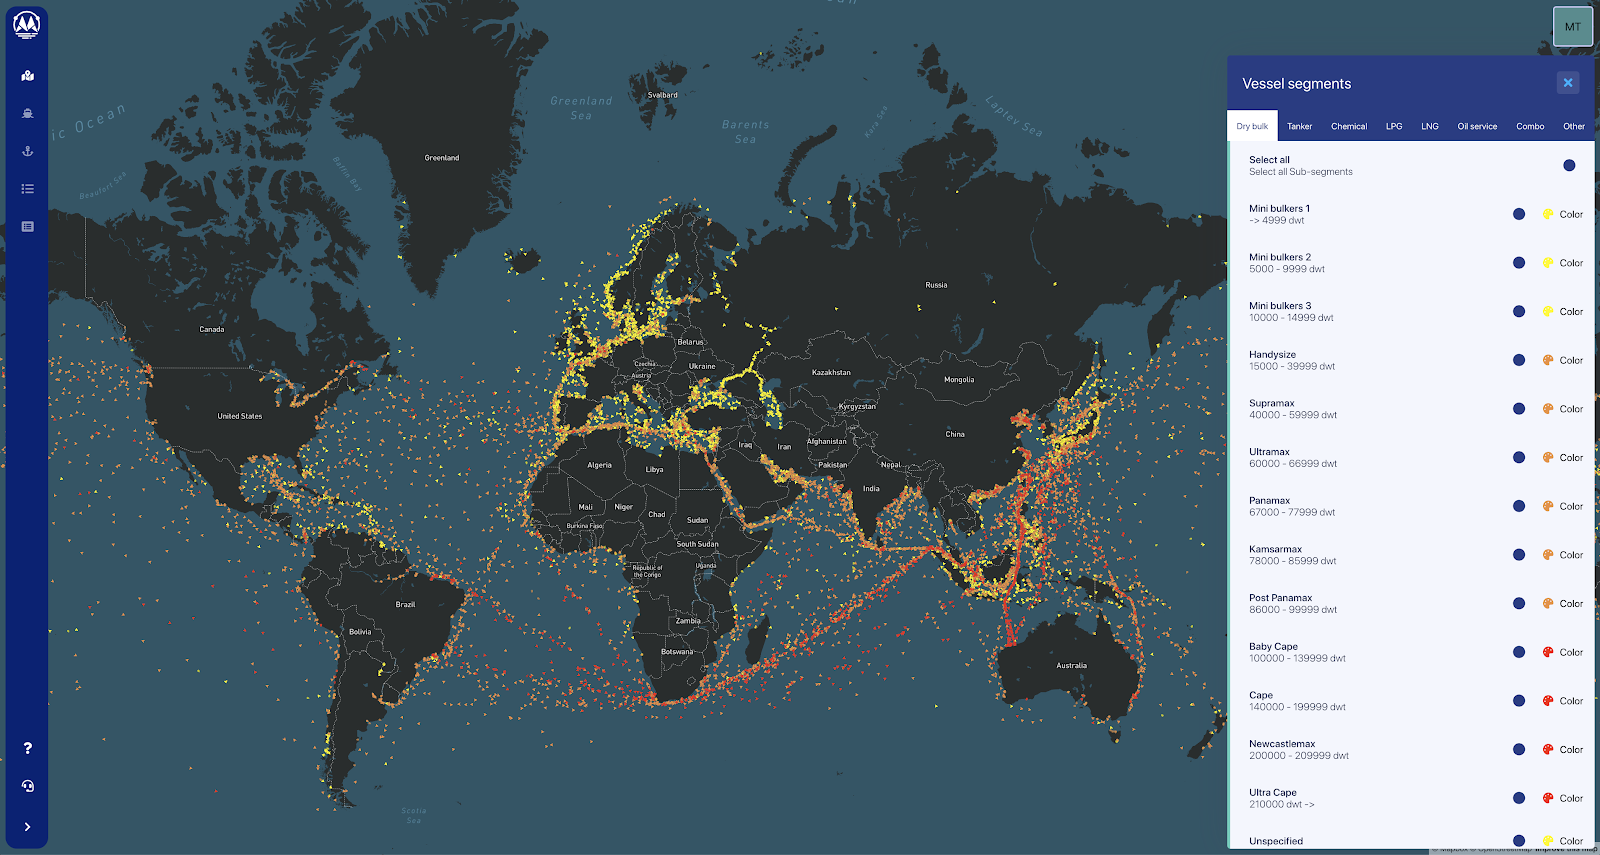
\includegraphics[width=1.0\textwidth]{figures/segment_map}
    \caption{\acrfull{mo}’s segmentation of vessels where yellow vessels are smaller than reds}
    \label{fig:segment_map}
\end{figure}

Moreover, \acrshort{mo} also has extensive vessel details for every vessel structured as a questionnaire in their product. This vast questionnaire contains information and fields from a combination of standards in the industry such as Q88\footnote{\url{https://corp.q88.com/}}. Data for the questionnaire is also collected from a number of external sources such as IHS Merkit\footnote{\url{https://ihsmarkit.com/index.html}} and DNV\footnote{\url{https://www.dnv.com/}}. Users of \acrshort{mo} also have the possibility of suggesting changes to a public version of this questionnaire for any vessel. These changes are verified by \acrshort{mo} and published if the information proves accurate. This detailed description of vessels provides creates a big potential for data analysis and a potential \acrshort{ml} model that is highly aware of specific vessels which ultimately may affect its traveling patterns. However, in this thesis, the main focus is on the vessel segmentation when developing the proposed solution. This data is later referred to as vessel segments and includes both the vessels' segment and sub-segment.

\subsection{Shipping ports}
\label{sec:shipping_ports}

\acrshort{mo} has an extensive port database containing more than 5600 ports. From sources such as UNECE it is possible to find a vast number of ports, however, only a sub-set of the worlds known ports are used by \acrshort{mo} as these are considered relevant shipping ports. The process of determining what ports are relevant shipping ports is a continuous manual process in \acrshort{mo} but it ensures that the available selection of ports is highly relevant for the industry. Furthermore, all ports are identified by their \gls{locode}. This is a five-letter unique identifier provided and managed by the United Nations (UN). In the five-letter code, the first two indicate the port's country of origin, while the three last indicate a more specific location within the origin country. As an example, the \gls{locode} for the port of Oslo is \texttt{NOOSL} where ``NO'' stands for Norway, and ``OSL'' stands for Oslo. For comparison, a similar system is used for international airports. For this thesis, only the 5600 relevant ports are considered for the analysis.
